% Chapter Template

\chapter{Results and Analysis} % Main chapter title

\label{c5} % Change X to a consecutive number; for referencing this chapter elsewhere, use \ref{ChapterX}

\section{Results and Analysis}

% Figure
% \begin{landscape}
%   \begin{figure*}[h!]
%     \centering
%       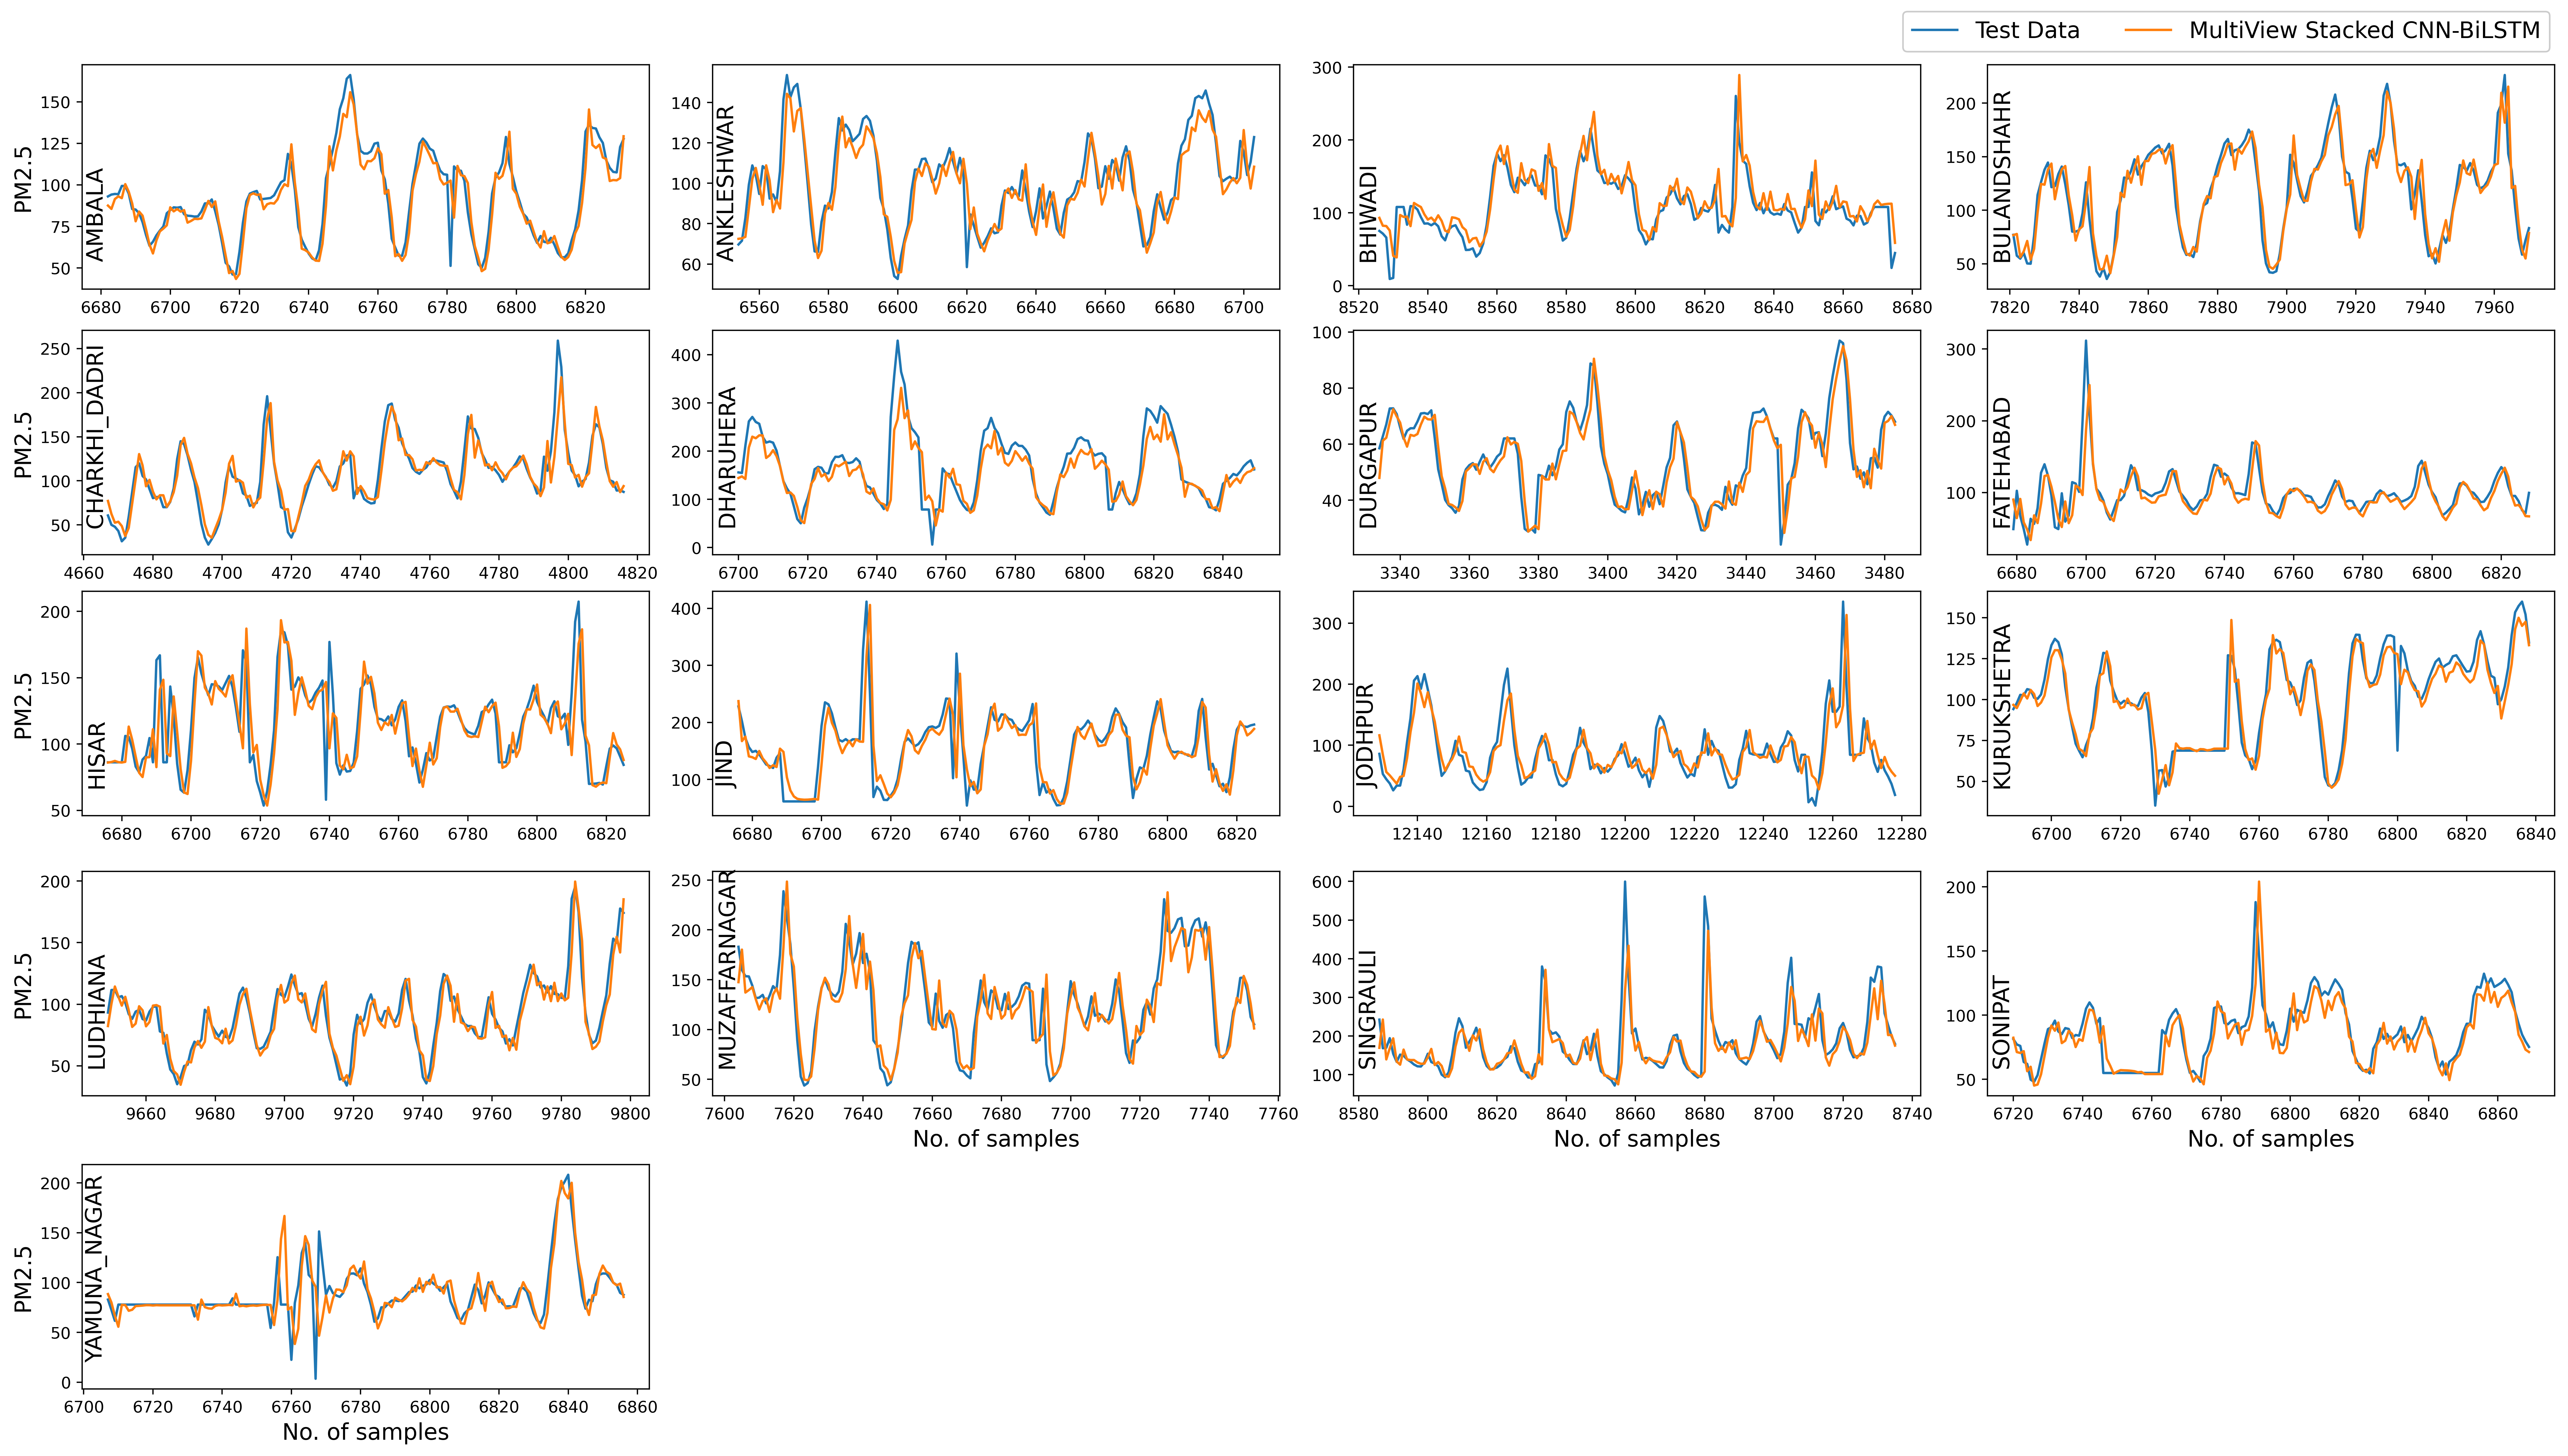
\includegraphics[scale=0.375]{act vs pri}
%       \caption{$PM_{2.5}$ predictions of proposed models MvS CNN-BiLSTM}\label{ACt_vs_Pred}
%   \end{figure*}
% \end{landscape}

\begin{figure*}
  \centering
  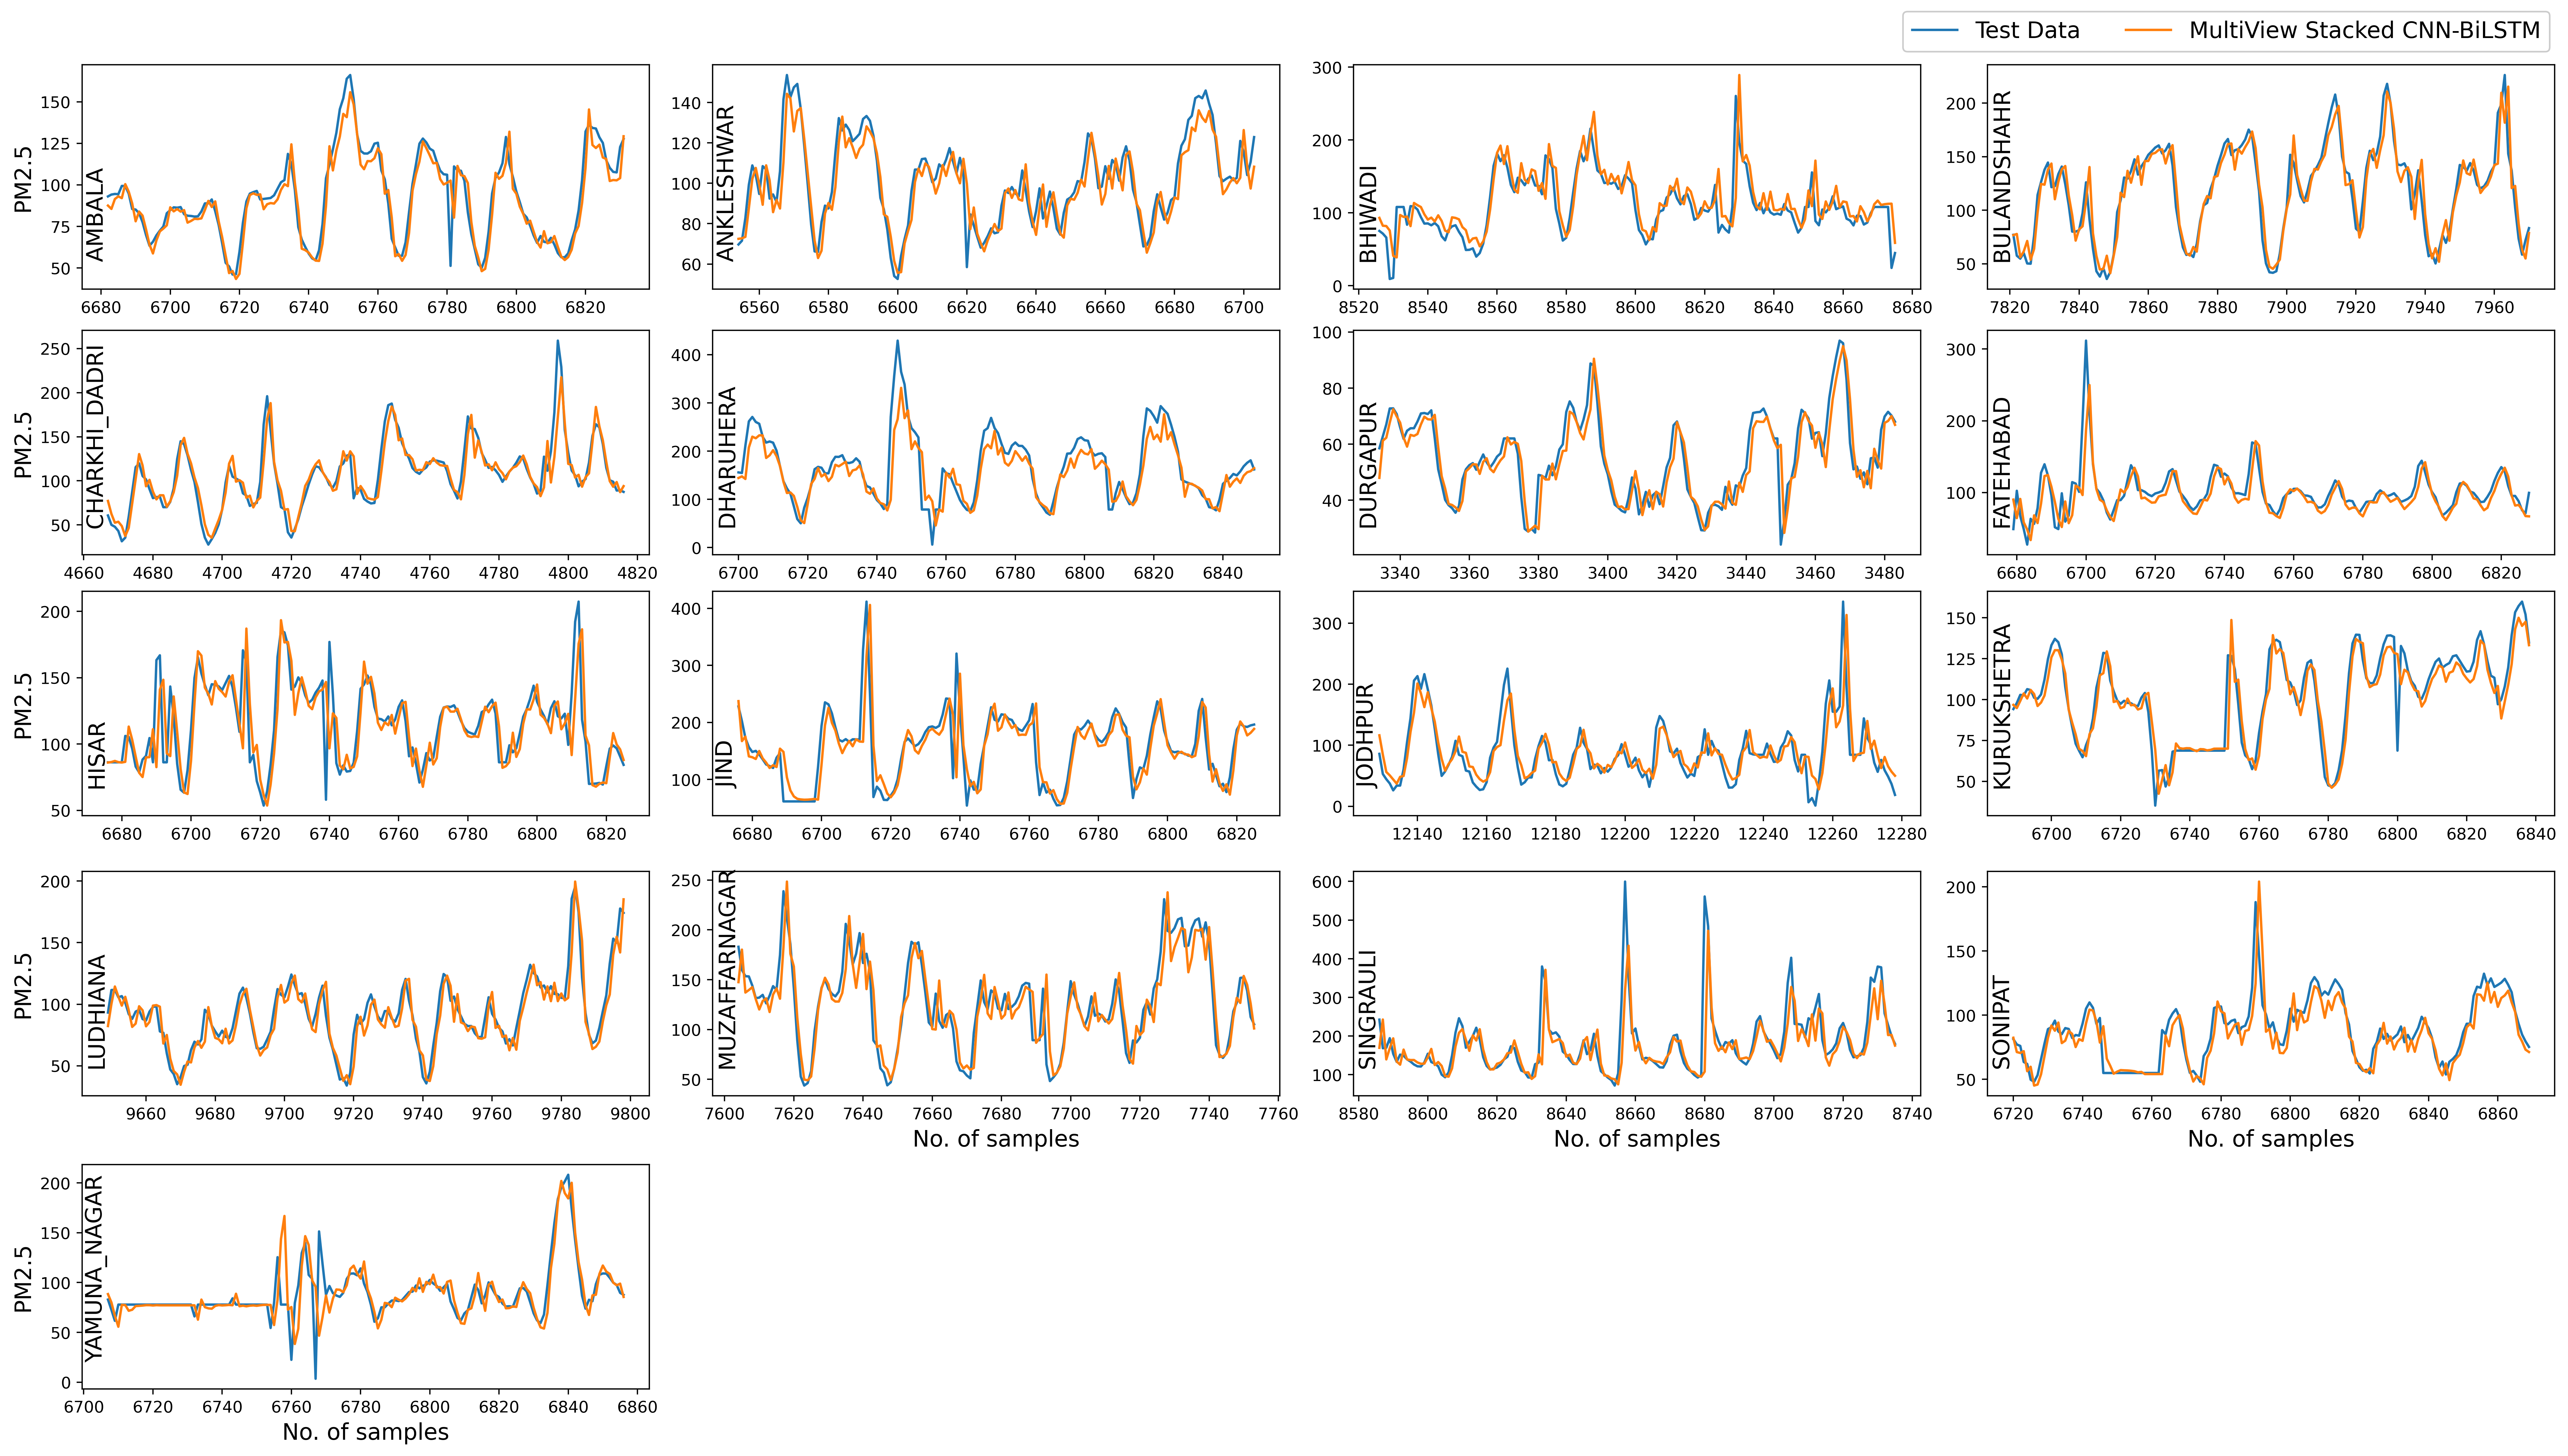
\includegraphics[scale=0.375]{act vs pri}
  \caption{$PM_{2.5}$ predictions of proposed models MvS CNN-BiLSTM}\label{ACt_vs_Pred}
\end{figure*}
\begin{figure*}
  \centering
  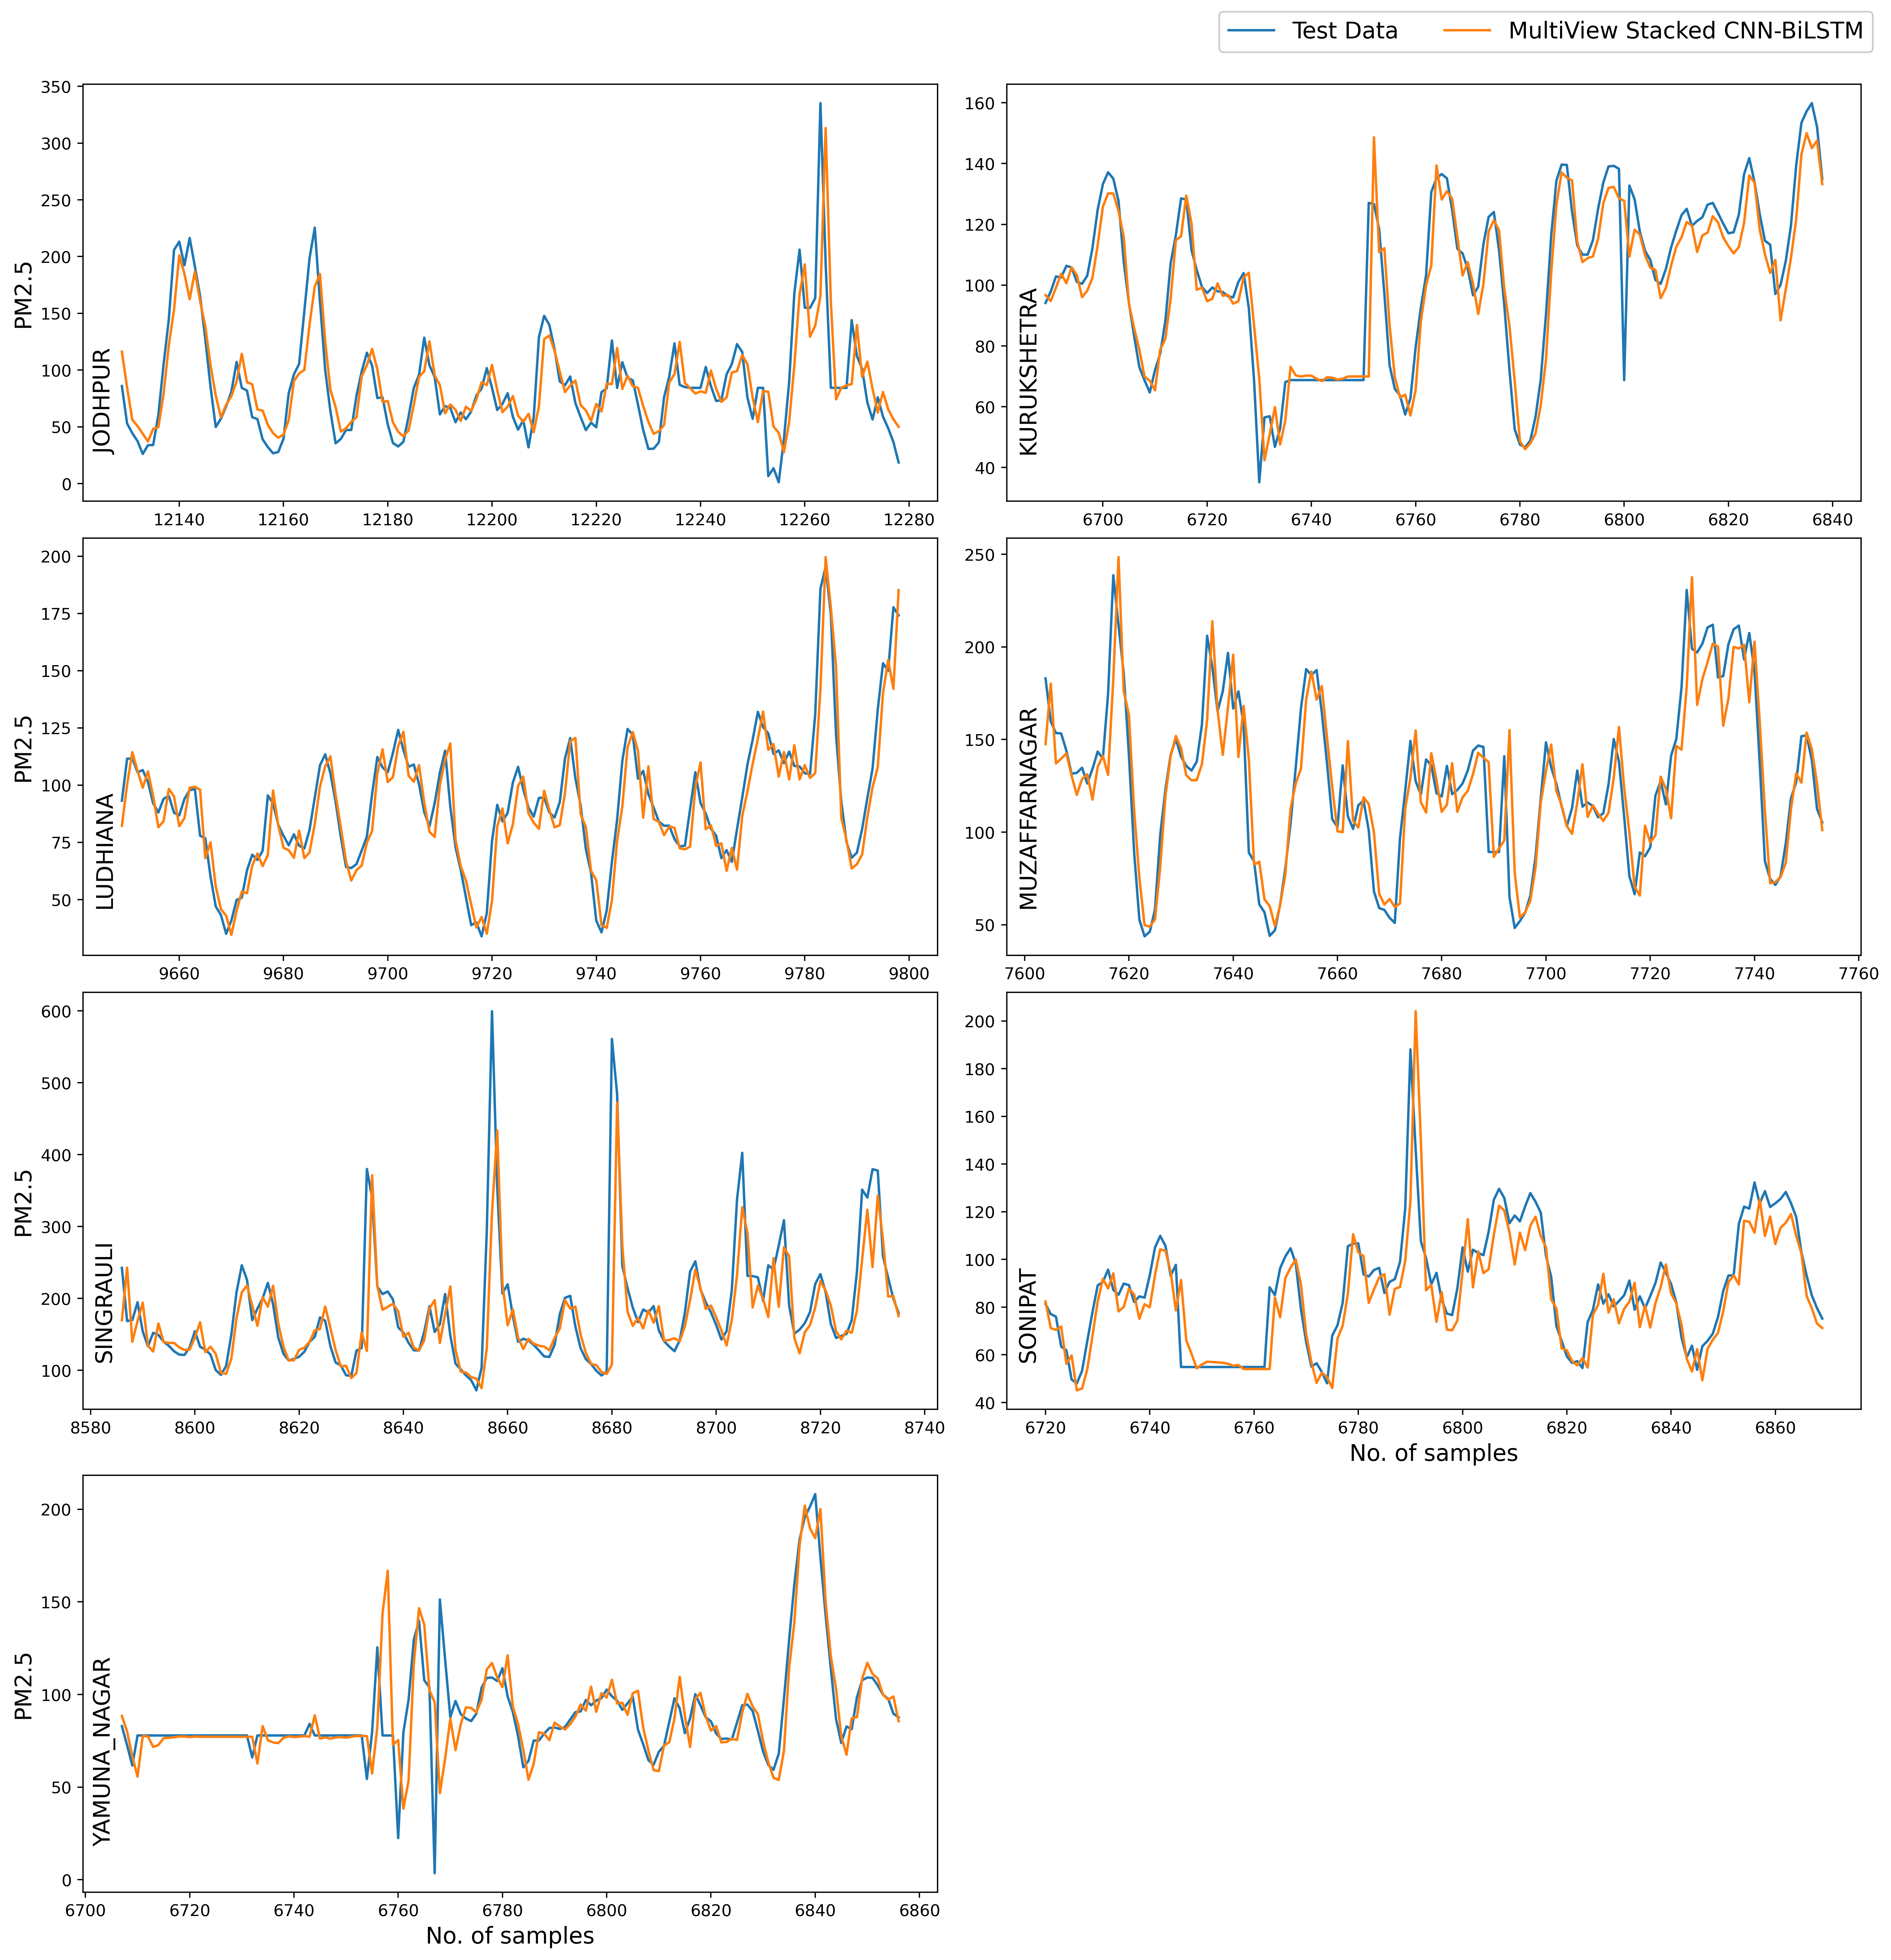
\includegraphics[scale=0.375]{act vs pri1}
  \caption{Continuation of $PM_{2.5}$ predictions of proposed models MvS CNN-BiLSTM}\label{ACt_vs_Pred1}
\end{figure*}
\Cref{ACt_vs_Pred,ACt_vs_Pred1} depicts a series of subplots that illustrate different datasets,  each showcasing the comparison between the predicted and actual $PM_{2.5}$ values on the test dataset. The x-axis indicates the quantity of data points,  while the $PM_{2.5}$ values are represented by the y-axis. Every subplot is associated with a specific dataset name,  signifying the MvS CNN-BiLSTM model's evaluation performance on various datasets,  which may reflect different periods or locations where $PM_{2.5}$ concentrations were monitored and documented. In each subplot,  the test dataset's samples are represented by data points. For each data point,  there are two values plotted:  the actual $PM_{2.5}$ value (ground truth) and the corresponding predicted $PM_{2.5}$ value generated by the MvS CNN-BiLSTM model. The plot allows us to visually compare how well the model's predictions match the actual values for each dataset. In \Cref{ACt_vs_Pred,ACt_vs_Pred}, the "prediction mimicking test" refers to comparing the model's predicted values with the actual values in the test dataset to assess the accuracy and effectiveness of the predictive model.





\begin{landscape}
    \setlength{\tabcolsep}{3pt}
  
    {\renewcommand{\arraystretch}{1}%
    \begin{longtable}[h!]{ p{0.22\linewidth} p{0.12\linewidth} p{0.07\linewidth} p{0.07\linewidth}  p{0.07\linewidth} p{0.07\linewidth} p{0.22\linewidth}  p{0.1\linewidth}}%{|l|l|l|l|l|l|}{llllllll}
        \caption{RMSE Performance of traditional DL models and proposed models $($ MvS CNN-BiLSTM$)$.}
        \label{tab: RMSE}\\
    \hline  DataSet        & BiLSTM  & CNN & GRU      & LSTM & RNN       & MvS CNN-BiLSTM        & Best-view \\ \hline
    \endhead
    %
    \hline
    \endfoot
    %
    \endlastfoot
    %
    AMBALA         & 33.382          & 36.239    & \textbf{33.012} & 33.136     & 33.455                & 33.272          & 4      \\
    ANKLESHWAR     & 22.916          & 23.724    & 22.975          & 23.359     & 22.807                & \textbf{22.081} & 6      \\
    BHIWADI        & 28.043          & 25.168    & 25.521          & 26.512     & 25.974                & \textbf{24.959} & 10     \\
    BULANDSHAHR    & 16.155          & 16.894    & \textbf{14.807} & 16.001     & 14.923                & 16.265          & 7      \\
     DCHARKHI\_DADRI & \textbf{30.071} & 32.709    & 32.299          & 32.629     & 33.836              & 31.064          & 3      \\
     DHARUHERA      & 25.751          & 26.948    & 26.057          & 26.108     & 25.489           &\textbf{24.983}          & 3      \\
     DURGAPUR       & 10.426          & 9.719     & 11.375          & 11.994     & 10.664                    & \textbf{8.906}  & 6      \\
     FATEHABAD      & 31.501          & 31.251    & 32.169          & 31.045     & 30.946                    & \textbf{30.86}  & 10     \\
     HISAR          & 21.677          & 22.286    & 20.875          & 21.371     & 21.617                 & \textbf{20.155} & 6      \\
     JIND           & 26.619          & 26.29     & 25.043          & 24.813     & \textbf{24.364}           & 24.408          & 10     \\
     JODHPUR        & 27.749          & 27.617    & 27.787          & 27.519     & 27.951              & \textbf{27.482} & 7      \\
     KURUKSHETRA    & 16.475          & 16.352    & 15.239          & 17.359     & \textbf{15.414}           & 15.921          & 5      \\
     LUDHIANA       & 14.573          & 17.013    & \textbf{13.817} & 17.668     & 14.936                    & 14.315          & 9      \\
     MUZAFFARNAGAR  & 20.885          & 23.182    & 21.206          & 20.412     & 23.638                   & \textbf{19.859} & 10     \\
     SINGRAULI      & 33.995          & 36.569    & \textbf{32.993} & 33.142     & 35.572                    & 33.834          & 2      \\
     SONIPAT        & 13.644          & 13.951    & 14.025          & 13.773     & 13.755                    & \textbf{12.75}  & 5      \\
     YAMUNA\_NAGAR  & 31.985          & 36.433    & 32.413          & 32.699     & 35.591                    & \textbf{31.676} & 8     \\ \hline
    \end{longtable}}
    \end{landscape}







  \Cref{tab: RMSE} exhibits the RMSE performance of different conventional DL models and the proposed MvS CNN-BiLSTM model on 17 datasets. The graph emphasises the random-performing model (i.e.,  the model with unpredictable RMSE) for each dataset using strikethrough text. The leftmost column lists the names of the evaluated datasets,  while the next columns represent the RMSE values of different traditional DL models on each dataset. The proposed MvS CNN-BiLSTM model's RMSE values are displayed in the "MvS CNN-BiLSTM" column. The "Best-view" column identifies the DL model that achieved the lowest RMSE on each dataset,  highlighted using bold text.

  The table thoroughly compares various DL models' RMSE performance across multiple datasets,  with the MvS CNN-BiLSTM model demonstrating better RMSE values in its respective column and the bolded values indicating the best-performing model for each dataset.
  
  \Cref{tab: RMSE} provides valuable insights into the predictive capabilities of traditional DL models and the proposed MvS CNN-BiLSTM model. The MvS CNN-BiLSTM model for better performance over several traditional deep learning models on diverse datasets,  as evidenced by the lower RMSE values. The highlighted values help identify the best model for each dataset,  highlighting the effectiveness of the proposed MvS CNN-BiLSTM approach over traditional DL models.
    \begin{table}[H]
        \setlength{\tabcolsep}{3pt}
        {\renewcommand{\arraystretch}{1}%
        \begin{longtable}[c]{ p{0.32\linewidth} p{0.12\linewidth} p{0.12\linewidth} p{0.12\linewidth}  p{0.12\linewidth} p{0.12\linewidth}}%{|l|l|l|l|}
        \caption{Percentage improvement of MvS CNN-BiLSTM respectively BiLSTM,  CNN,  GRU,  LSTM and RNN on RMSE.}
        \label{RMSE imp}
        \\ \hline
        Dataset        &   BiLSTM &   CNN &   GRU &   LSTM &   RNN 
        \\ \hline
        \endhead
        %
        AMBALA & 0.33\% & 8.19\% & -0.79 \% & -0.41\% & 0.55\% \\
        ANKLESHWAR & 3.64\% & 6.93\% & 3.89\% & 5.47\% & 3.18\% \\
        BHIWADI & 11.00\% & 0.83\% & 2.20\% & 5.86\% & 3.91\% \\
        BULANDSHAHR & -0.68\% & 3.72\% & -9.85\% & -1.65\% & -8.99\% \\
        CHARKHI\_DADRI &-3.3\% & 5.03\% & 3.82\% & 4.80\% & 8.19\% \\
        DHARUHERA & 2.98\% & 7.29\% & 4.12\% & 4.31\% & 1.99\% \\
        DURGAPUR & 14.58\% & 8.37\% & 21.71\% & 25.75\% & 16.49\% \\
        FATEHABAD & 2.03\% & 1.25\% & 4.07\% & 0.60\% & 0.28\% \\
        HISAR & 7.02\% & 9.56\% & 3.45\% & 5.69\% & 6.76\% \\
        JIND & 8.31\% & 7.16\% & 2.54\% & 1.63\% & -0.18\% \\
        JODHPUR & 0.96\% & 0.49\% & 1.10\% & 0.13\% & 1.68\% \\
        KURUKSHETRA & 3.36\% & 2.64\% & -4.48\% & 8.28\% & -3.29\% \\
        LUDHIANA & 1.77\% & 15.86\% & -3.6\% & 18.98\% & 4.16\% \\
        MUZAFFARNAGAR & 4.91\% & 14.33\% & 6.35\% & 2.71\% & 15.99\% \\
        SINGRAULI & 0.47\% & 7.48\% & -2.55\% & -2.09\% & 4.89\% \\
        SONIPAT & 6.55\% & 8.61\% & 9.09\% & 7.43\% & 7.31\% \\
        YAMUNA\_NAGAR & 0.97\% & 13.06\% & 2.27\% & 3.13\% & 11.00\% \\ \hline
        \textbf{Positive Avg}  & \textbf{4.05\%} & \textbf{7.11\%}& \textbf{3.80\%} & \textbf{5.57\%} & \textbf{5.08\%} \\ \hline
        \end{longtable}}
        
        \end{table}


  \Cref{RMSE imp} illustrates the extent $\%$ of improvement from conventional deep learning (DL) models to the proposed MvS CNN-BiLSTM model across 17 datasets. The chart showcases the growth rate of every deep learning model,  namely BiLSTM,  CNN,  GRU,  LSTM,  and RNN, concerning the MvS CNN-BiLSTM model. Negative values indicate that the corresponding DL model outperformed the MvS CNN-BiLSTM model for a particular dataset. The table consists of a pair of columns that are connected. The right column denotes the percentage improvement of the MvS CNN-BLSTM model compared to traditional DL models for each dataset evaluated, as shown in the left columns.  A positive percentage value denotes that the MvS CNN-BiLSTM model performed better than the DL model.



% \begin{table}[!htp]
%   \caption{Average Rankings of the algorithms (Friedman) in a contest of RMSE.}
%   \centering
%   \begin{tabular}{lccc}
%   \hline
%   Algorithm&Ranking&$p$&Holm\\\hline
%   BiLSTM&3.7059&0.002485&0.016667\\
%   CNN&4.8235&0.000002&0.01\\
%   GRU&3.1765&0.027801&0.05\\
%   LSTM&3.8235&0.001335&0.0125\\
%   RNN&3.7059&0.002485&0.025\\
%   \textbf{MvS CNN-BiLSTM}&\textbf{1.7647}&$-$ &$-$ \\\hline
% \end{tabular}
% \label{rank_rmse}
%   \end{table}


  \begin{table}[H]
    \setlength{\tabcolsep}{3pt}
    {\renewcommand{\arraystretch}{1}%
    \begin{longtable}[c]{ p{0.35\linewidth} p{0.20\linewidth} p{0.20\linewidth} p{0.20\linewidth}  }
      \caption{Average Rankings of the algorithms (Friedman) in a contest of RMSE.}
      \label{rank_rmse}
    \\ \hline
    Algorithm&Ranking&$p$&Holm
    \\ \hline
    \endhead
    %
    BiLSTM&3.7059&0.002485&0.016667\\
    CNN&4.8235&0.000002&0.01\\
    GRU&3.1765&0.027801&0.05\\
    LSTM&3.8235&0.001335&0.0125\\
    RNN&3.7059&0.002485&0.025\\
    \textbf{MvS CNN-BiLSTM}&\textbf{1.7647}&$-$ &$-$ \\\hline
    \end{longtable}}
    \end{table}





  \Cref{rank_rmse} exhibits the average rankings of various algorithms about the RMSE metric,  thereby providing insights into their relative performance. The table comprises four columns: algorithm,  Ranking,  $p$-value,  and Holm. The names of several algorithms,  including BiLSTM,  CNN,  GRU,  LSTM,  RNN,  and the recently suggested MvS CNN-BiLSTM,  are being logged in the algorithm column while the assessment process is underway. The standing column exhibits the mean ranks of every algorithm relying on their performance in terms of RMSE,  where a lesser rank indicates superior performance, with 1 being the best rank and higher numbers indicating weaker performance. Each algorithm's comparison is assigned a significance level in the $p$-value column,  with a small $p$-value indicating a statistically significant difference in performance between the compared algorithms. The Holm column controls the family-wise error rate by indicating adjusted significance thresholds utilised in multiple statistical tests. The proposed MvS CNN-BiLSTM algorithm accomplished an average ranking of 1.7647, the finest among all compared models concerning RMSE. The MvS CNN-BiLSTM algorithm was not used in comparing traditional shallow learning models (BiLSTM,  CNN,  GRU,  LSTM,  and RNN). Furthermore,  the minute $p$-values for every algorithmic comparison imply a statistically significant variance in performance amongst all the algorithms,  signifying that the performance of each algorithm is discernible from others based on the RMSE metric. The Holm column likely indicates the adjusted significance thresholds (critical values) used in the Holm method for multiple comparisons, a statistical procedure used to control the family-wise error rate when performing multiple hypothesis tests. The MvS CNN-BiLSTM algorithm is the superior choice based on the table's data,  performing better than other algorithms in RMSE.






  \begin{landscape}
    \setlength{\tabcolsep}{3pt}
  
    {\renewcommand{\arraystretch}{1}%
    \begin{longtable}[h!]{ p{0.22\linewidth} p{0.12\linewidth} p{0.07\linewidth} p{0.07\linewidth}  p{0.07\linewidth} p{0.07\linewidth} p{0.22\linewidth}  p{0.1\linewidth}}%{|l|l|l|l|l|l|}{llllllll}
      \caption{MAPE Performance of traditional DL models and proposed models $($MvS CNN-BiLSTM$)$.}
      \label{tab: MAPE}\\
    \hline  DataSet        & BiLSTM  & CNN & GRU      & LSTM & RNN      & MvS CNN-BiLSTM        & Best-view \\ \hline
    \endhead
    %
    \hline
    \endfoot
    %
    \endlastfoot
    %
    AMBALA         & 54.468       & 49.153    & 76.839    & 58.619     & 53.375    & \textbf{18.73}  & 3      \\
    ANKLESHWAR     & 18.86        & 19.968    & 19.015    & 19.576     & 20.72     & \textbf{16.265} & 10     \\
    BHIWADI        & 134.448      & 118.741   & 123.123   & 127.481    & 124.503   & \textbf{20.98}  & 2      \\
    BULANDSHAHR    & 44.602       & 47.066    & 26.254    & 43.721     & 27.813    & \textbf{22.469} & 3      \\
    CHARKHI\_DADRI & 50.328       & 101.385   & 102.063   & 112.912    & 115.673   & \textbf{26.728} & 10     \\
    DHARUHERA      & 35.638       & 39.358    & 39.557    & 35.942     & 40.34     & \textbf{17.365} & 3      \\
    DURGAPUR       & 45.511       & 37.529    & 56.324    & 57.457     & 48.626    & \textbf{19.321} & 6      \\
    FATEHABAD      & 19.737       & 19.929    & 19.475    & 18.663     & 17.724    & \textbf{12.178} & 5      \\
    HISAR          & 17.971       & 18.422    & 17.988    & 17.983     & 21.475    & \textbf{15.082} & 6      \\
    JIND           & 25.945       & 30.822    & 27.344    & 24.596     & 33.464    & \textbf{16.618} & 3      \\
    JODHPUR        & 40.188       & 40.36     & 41.584    & 41.578     & 43.36     & \textbf{28.278} & 7      \\
    KURUKSHETRA    & 13.713       & 13.392    & 12.405    & 13.986     & 13.312    & \textbf{11.248} & 2      \\
    LUDHIANA       & 37.61        & 47.14     & 34.504    & 51.036     & 41.197    & \textbf{15.706} & 9      \\
    MUZAFFARNAGAR  & 24.162       & 27.253    & 23.37     & 26.08      & 27.061    & \textbf{16.571} & 5      \\
    SINGRAULI      & 48.642       & 67.143    & 39.738    & 34.372     & 68.525    & \textbf{28.545} & 7      \\
    SONIPAT        & 43.301       & 48.32     & 49.409    & 43.187     & 45.67     & \textbf{13.541} & 7      \\
    YAMUNA\_NAGAR  & 65.601       & 63.698    & 64.637    & 63.404     & 70.02     & \textbf{28.29}  & 10    \\ \hline
    \end{longtable}}
    \end{landscape}

\Cref{tab: MAPE} showcases MAPE results of the MvS CNN-BiLSTM model and traditional DL models across 17 datasets. The DL models analysed in the table include BiLSTM,  CNN,  GRU,  LSTM,  and RNN. The MAPE values for each DL model are compared with those of the MvS CNN-BiLSTM model. The minimum MAPE values obtained by each model for each dataset and the corresponding best view are presented in \textbf{bold}. To expound the \Cref{tab: MAPE},  the initial column enumerates the names of the datasets assessed in the investigation. The succeeding columns indicate the MAPE values for the different traditional DL models compared to each dataset's proposed MvS CNN-BiLSTM model. The table's interpretation involves the presentation of the corresponding MAPE value for each DL model to their respective columns. The "Best-view" column,  on the other hand,  specifies the best dataset for which the MvS CNN-BiLSTM model obtained the minimum MAPE value. In conclusion,  \Cref{tab: MAPE} compares the MAPE performance of the MvS CNN-BiLSTM model and traditional DL models across multiple datasets. The values in \textbf{bold} highlight the MvS CNN-BiLSTM model's superior performance over traditional DL models for different datasets. The table demonstrates the MvS CNN-BiLSTM model's ability to reduce MAPE for air quality prediction in various locations and datasets.



\begin{table}[H]
  \setlength{\tabcolsep}{3pt}
  {\renewcommand{\arraystretch}{1}%
  \begin{longtable}[c]{ p{0.32\linewidth} p{0.12\linewidth} p{0.12\linewidth} p{0.12\linewidth}  p{0.12\linewidth} p{0.12\linewidth}}%{|l|l|l|l|}
    \caption{ Improvement of MvS CNN-BiLSTM respectively BiLSTM,  GRU,  LSTM and RNN on MAPE.}
    \label{MAPE imp}
  \\ \hline
  Dataset       &   BiLSTM &CNN & GRU &   LSTM &   RNN 
  \\ \hline
  \endhead
  %
  AMBALA & 35.74\% & 30.42\% & 58.11\% & 39.89\% & 34.64\% \\
  ANKLESHWAR & 2.59\% & 3.70\% & 2.75\% & 3.31\% & 4.45\% \\
  BHIWADI & 113.47\% & 97.76\% & 102.14\% & 106.50\% & 103.52\% \\
  BULANDSHAHR & 22.13\% & 24.60\% & 3.78\% & 21.25\% & 5.34\% \\
  CHARKHI\_DADRI & 23.60\% & 74.66\% & 75.34\% & 86.18\% & 88.94\% \\
  DHARUHERA & 18.27\% & 21.99\% & 22.19\% & 18.58\% & 22.98\% \\
  DURGAPUR & 26.19\% & 18.21\% & 37.00\% & 38.14\% & 29.30\% \\
  FATEHABAD & 7.56\% & 7.75\% & 7.30\% & 6.48\% & 5.55\% \\
  HISAR & 2.89\% & 3.34\% & 2.91\% & 2.90\% & 6.39\% \\
  JIND & 9.33\% & 14.20\% & 10.73\% & 7.98\% & 16.85\% \\
  JODHPUR & 11.91\% & 12.08\% & 13.31\% & 13.30\% & 15.08\% \\
  KURUKSHETRA & 2.46\% & 2.14\% & 1.16\% & 2.74\% & 2.06\% \\
  LUDHIANA & 21.90\% & 31.43\% & 18.80\% & 35.33\% & 25.49\% \\
  MUZAFFARNAGAR & 7.59\% & 10.68\% & 6.80\% & 9.51\% & 10.49\% \\
  SINGRAULI & 20.10\% & 38.60\% & 11.19\% & 5.83\% & 39.98\% \\
  SONIPAT & 29.76\% & 34.78\% & 35.87\% & 29.65\% & 32.13\% \\
  YAMUNA\_NAGAR & 37.31\% & 35.41\% & 36.35\% & 35.11\% & 41.73\% \\ \hline
  \textbf{Positive Avg} & \textbf{23.11\% }& \textbf{27.16\% }& \textbf{26.22\%} & \textbf{27.22\%} & \textbf{28.52\%} \\ \hline
  \end{longtable}}
  \end{table}
\Cref{MAPE imp} displays the percentage improvement in MAPE attained by the proposed MvS CNN-BiLSTM model compared to various traditional DL models (BiLSTM,  GRU,  LSTM,  RNN) for all 17 datasets. The first column of the table lists the names of the datasets evaluated in the study. The succeeding columns represent the percentage improvement in MAPE achieved by the MvS CNN-BiLSTM model over each traditional DL model on each dataset. The percentage values in the table indicate the reduction in MAPE attained by the MvS CNN-BiLSTM model relative to each traditional DL model,  with negative values implying cases where the traditional DL model outperformed the MvS CNN-BiLSTM model.



    \begin{table}[H]
      \setlength{\tabcolsep}{3pt}
      {\renewcommand{\arraystretch}{1}%
      \begin{longtable}[c]{ p{0.35\linewidth} p{0.20\linewidth} p{0.20\linewidth} p{0.20\linewidth}  }
        \caption{Average rankings of the algorithms (Friedman) in the context of MAPE.}
        \label{rank_mape}
      \\ \hline
      Algorithm&Ranking&$p$&Holm
      \\ \hline
      \endhead
      %
      BiLSTM&3.4706&0.000118&0.05\\
      CNN&4.1765&0.000001&0.0125\\
      GRU&3.7647&0.000016&0.025\\
      LSTM&3.8824&0.000007&0.016667\\
      RNN&4.7059&0&0.01\\
      \textbf{MvS CNN-BiLSTM}&\textbf{1}&$-$ &$-$\\\hline
      \end{longtable}}
      \end{table}


      \Cref{rank_mape} showcases the average rankings of multiple algorithms in the context of the MAPE metric,  providing insight into the relative performance of these algorithms. The primary row comprises the appellation of the systems being measured,  particularly BiLSTM,  CNN,  GRU,  LSTM,  RNN,  and the purpose of MvS CNN-BiLSTM. The subsequent column displays the average rankings of each algorithm according to their MAPE performance,  with a lower ranking indicating superior performance and a greater number indicating inferior performance. The third column denotes the p-values, the significance level for comparing each algorithm. A statistically significant difference in performance between the compared algorithms is present if the $p$-value is low. The fourth column,  "Holm, " will likely denote the critical values or adjusted significance thresholds used for multiple comparisons. The Holm method manages the family-wise error rate when conducting multiple statistical tests.
      
      The MvS CNN-BiLSTM algorithm is better regarding MAPE,  surpassing all other models,  including BiLSTM,  CNN,  GRU,  LSTM,  and RNN,  with an average rank of 1. It is thus improbable to assume that any other compared algorithm outperforms the MvS CNN-BiLSTM algorithm regarding MAPE. Furthermore,  the small $p$-values for every algorithmic comparison indicate statistically significant efficacy disparities among all algorithms. This implies that the algorithms' performance is distinguishable from one another based on the MAPE metric. The "Holm" column likely denotes the adjusted significance thresholds (critical values) used in the Holm method for multiple comparisons. The Holm method is a statistical technique employed for controlling family-wise error rates during the execution of multiple hypothesis tests. In summary,  \Cref{rank_mape} shows that the proposed MvS CNN-BiLSTM algorithm is the best among all the compared algorithms in terms of MAPE. Moreover, statistically meaningful performance distinctions exist among the MAPE metric-based algorithms.
    



% Figure
\begin{figure}[ht]
	\centering
		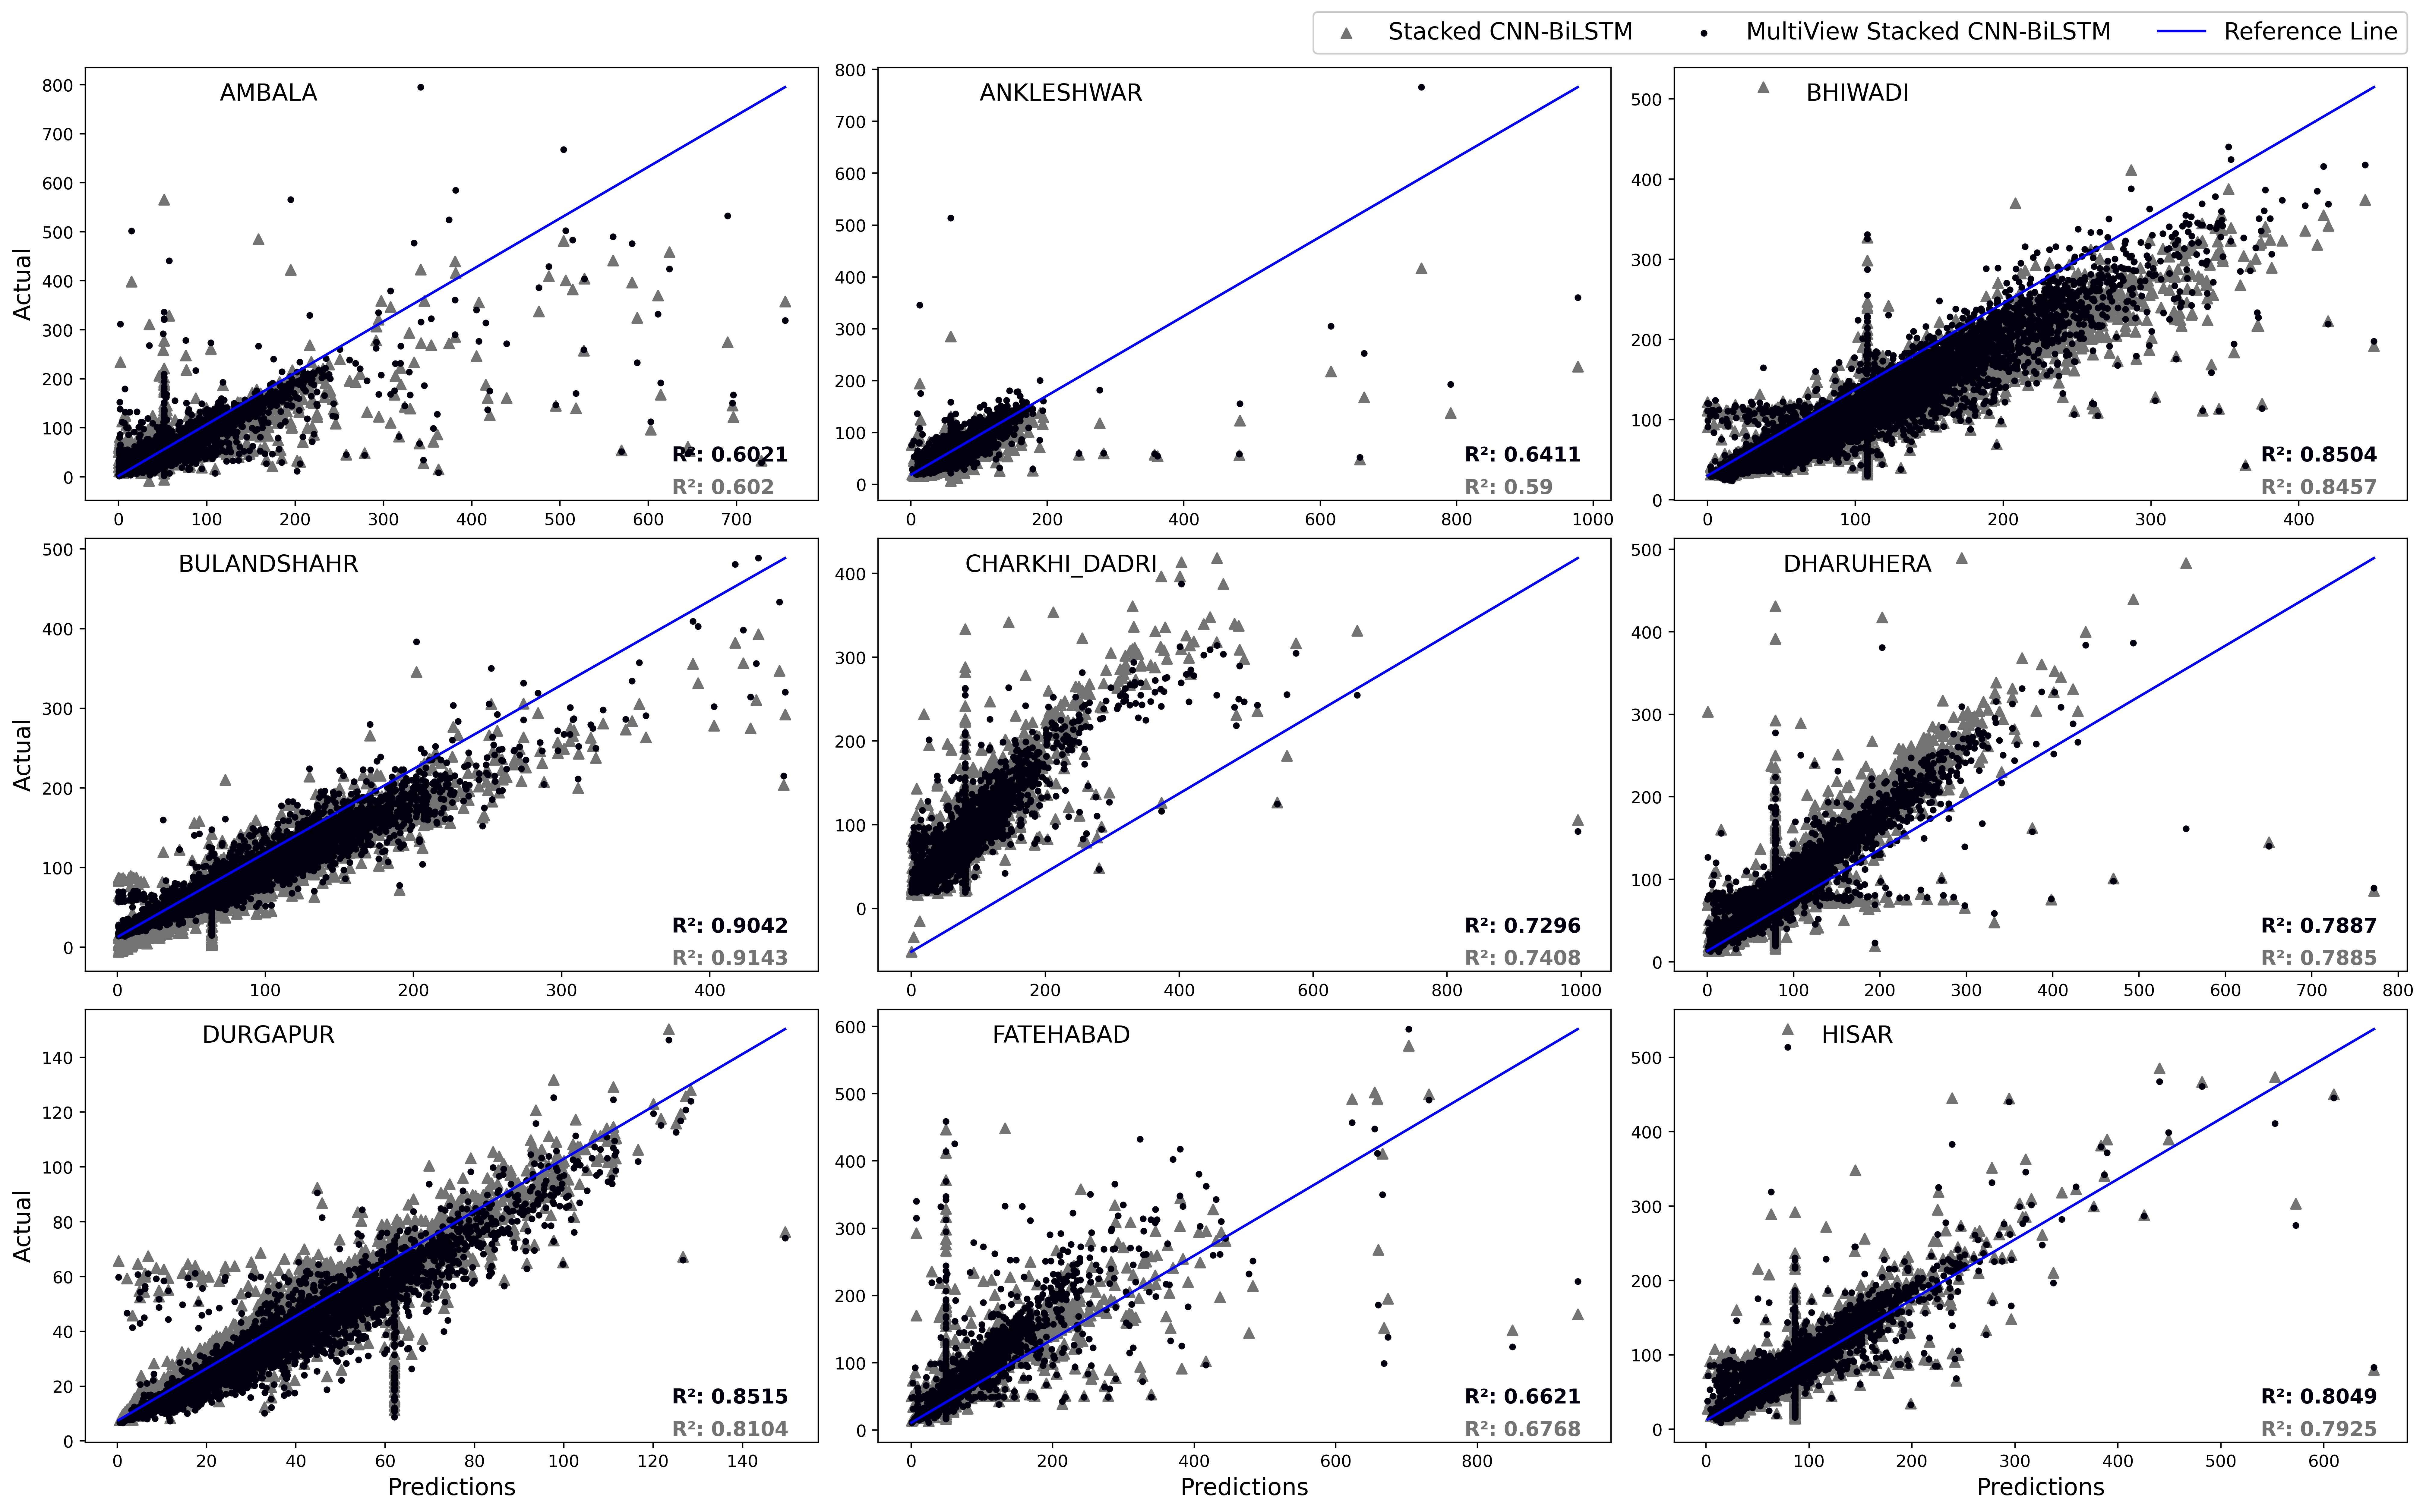
\includegraphics[scale=0.375]{Scatter_plot}
	  \caption{Correlation of Actual values and Predictions of proposed models $($Stacked CNN-BiLSTM and MvS CNN-BiLSTM $)$ using Scatter plot.}\label{Scatter}
\end{figure}
\begin{figure}[ht]
	\centering
		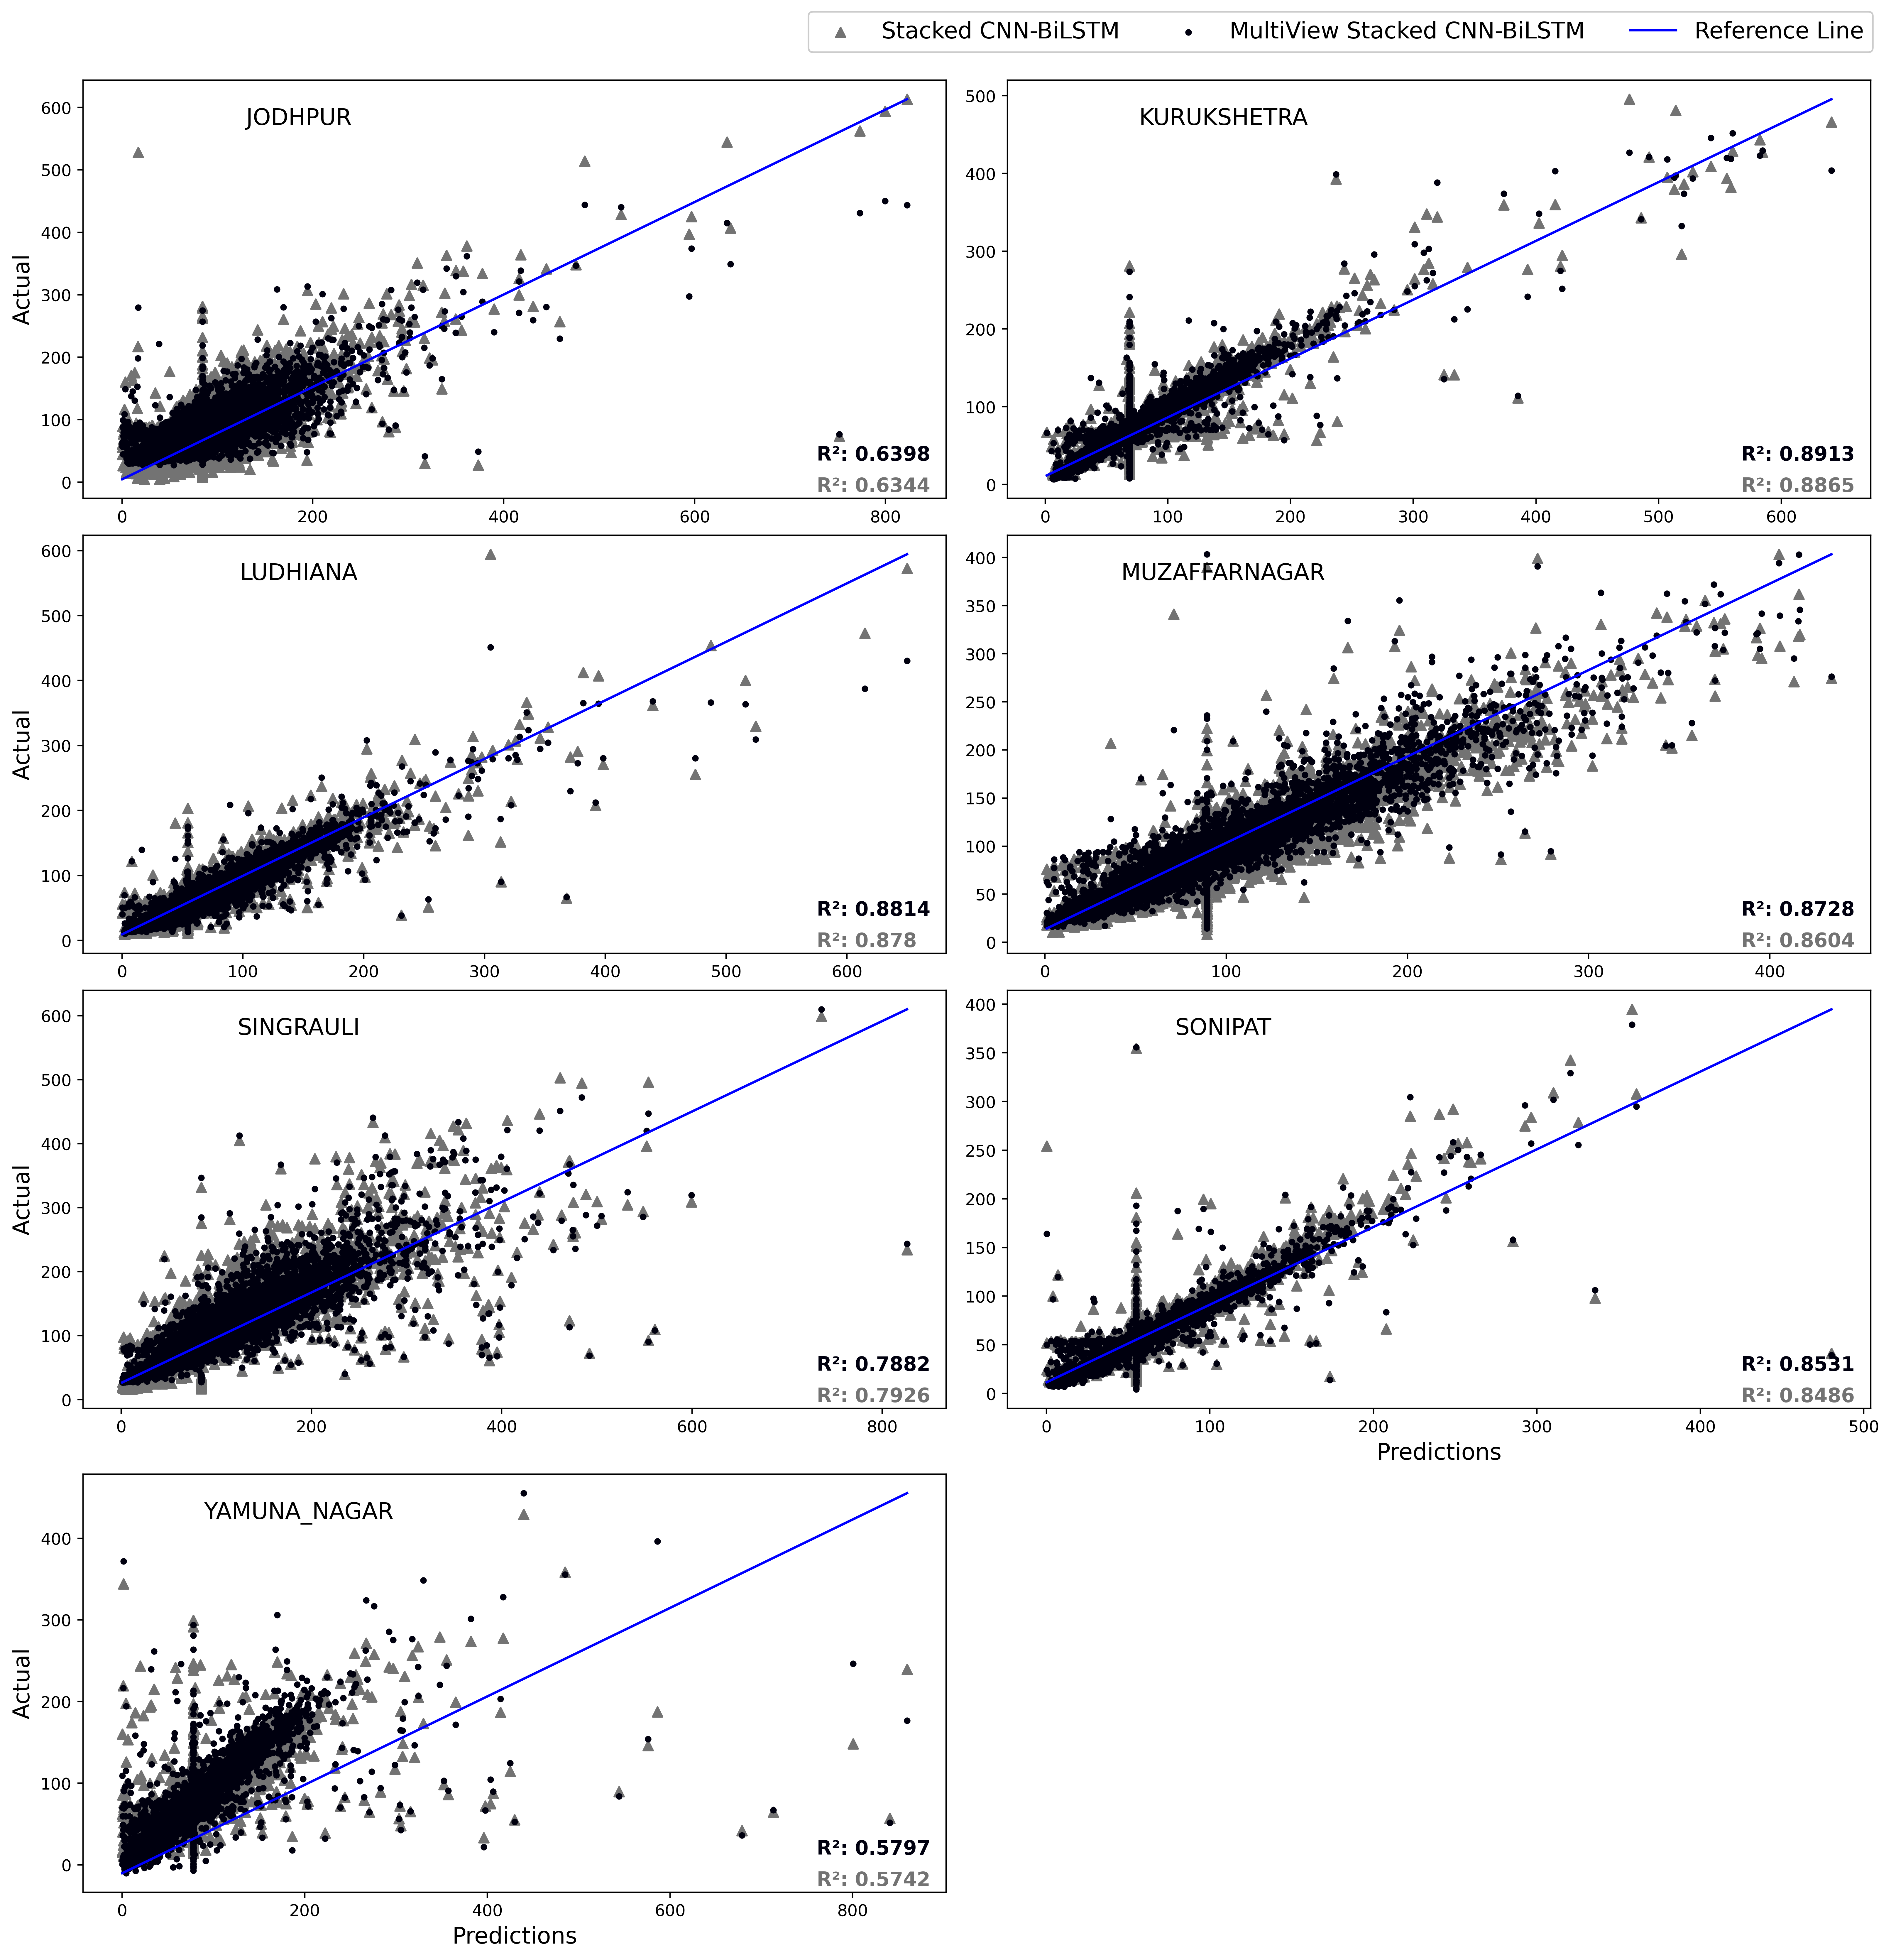
\includegraphics[scale=0.375]{Scatter_plot1}
	  \caption{Continuation of Correlation of Actual values and Predictions of proposed models $($Stacked CNN-BiLSTM and MvS CNN-BiLSTM $)$ using Scatter plot.}\label{Scatter1}
\end{figure}
The \Cref{Scatter,Scatter1} contains 17 subplots,  each displaying a scatter plot for multiple datasets,  and compares the grey Stacked CNN-BiLSTM model with the black Proposed MvS CNN-BiLSTM model. The plot includes a blue reference line representing the optimal scenario in which predicted and actual values are aligned. Additionally,  each subplot displays two $R^2$ values corresponding to the grey and black superimposed plots. A heightened $R^2$ value suggests a more powerful correlation between anticipated and actual values,  making it a valuable statistical gauge of fitness in provided Figure; there are two potential interpretations:  If the grey Stacked CNN-BiLSTM has a more excellent $R^2$ value than the black Proposed MvS CNN-BiLSTM,  The analysis shows that the grey model had superior accuracy and a more resilient correlation between projected and actual values than the black model,  leading to a superior overall fit. The same $R^2$ value of the black Proposed MvS CNN-BiLSTM and the grey Stacked CNN-BiLSTM makes it irrelevant which model performed better in predicting actual values and has a similar goodness-of-fit and correlation with actual values. Based on the information you provided,  it appears that for the \Cref{Scatter,Scatter1} Singrauli,  Fatehabad,  Charkhi\_Dadri,  and Bulandshahr,  the grey Stacked CNN-BiLSTM model has higher $R^2$ values compared to the black Proposed MvS CNN-BiLSTM model. However,  you mentioned that the $R^2$ values for the black model are very close to the grey model. In this case,  since the $R^2$ values for the black model are very close to the grey model,  it suggests that both models have similar predictive performance for those datasets. The difference in their $R^2$ values might be slight,  indicating that they are both relatively accurate in predicting the actual values. It has concluded that the association of multi-view leading with stacked CNN-BiLSTM is performing better than the stacked CNN-BiLSTM along with the traditional model over various measures.


% \begin{table}[!htp]
%   \caption{Overall average of RMSE and MAPE ranking of traditional models and proposed model (MvS CNN-BiLSTM).}
%   \centering
%   \begin{tabular}{lccc}
%   \hline
%   Algorithm&RMSE\_Ranking&MAPE\_Ranking&Average\_Ranking\\\hline
%   BiLSTM&3.7059&3.4706&3.58825\\
%   CNN&4.8235&4.1765&4.5\\
%   GRU&3.1765&3.7647&3.4706\\
%   LSTM&3.8235&3.8824&3.85295\\
%   RNN&3.7059&4.7059&4.2059\\
%   \textbf{MvS CNN-BiLSTM}&\textbf{1.7647}&\textbf{1}&\textbf{1.38235} \\\hline
% \end{tabular}
% \label{AVG RANK}
%   \end{table}




  \begin{table}[H]
    \setlength{\tabcolsep}{3pt}
    {\renewcommand{\arraystretch}{1}%
    \begin{longtable}[c]{ p{0.35\linewidth} p{0.20\linewidth} p{0.20\linewidth} p{0.20\linewidth}  }
      \caption{Overall average of RMSE and MAPE ranking of traditional models and proposed model (MvS CNN-BiLSTM).}
      \label{AVG RANK}
    \\ \hline
    Algorithm&RMSE\_Ranking&MAPE\_Ranking&Average\_Ranking
    \\ \hline
    \endhead
    %
    BiLSTM&3.7059&3.4706&3.58825\\
    CNN&4.8235&4.1765&4.5\\
    GRU&3.1765&3.7647&3.4706\\
    LSTM&3.8235&3.8824&3.85295\\
    RNN&3.7059&4.7059&4.2059\\
    \textbf{MvS CNN-BiLSTM}&\textbf{1.7647}&\textbf{1}&\textbf{1.38235} \\\hline
    \end{longtable}}
    \end{table}







  \begin{figure*}[h!]
    \centering
    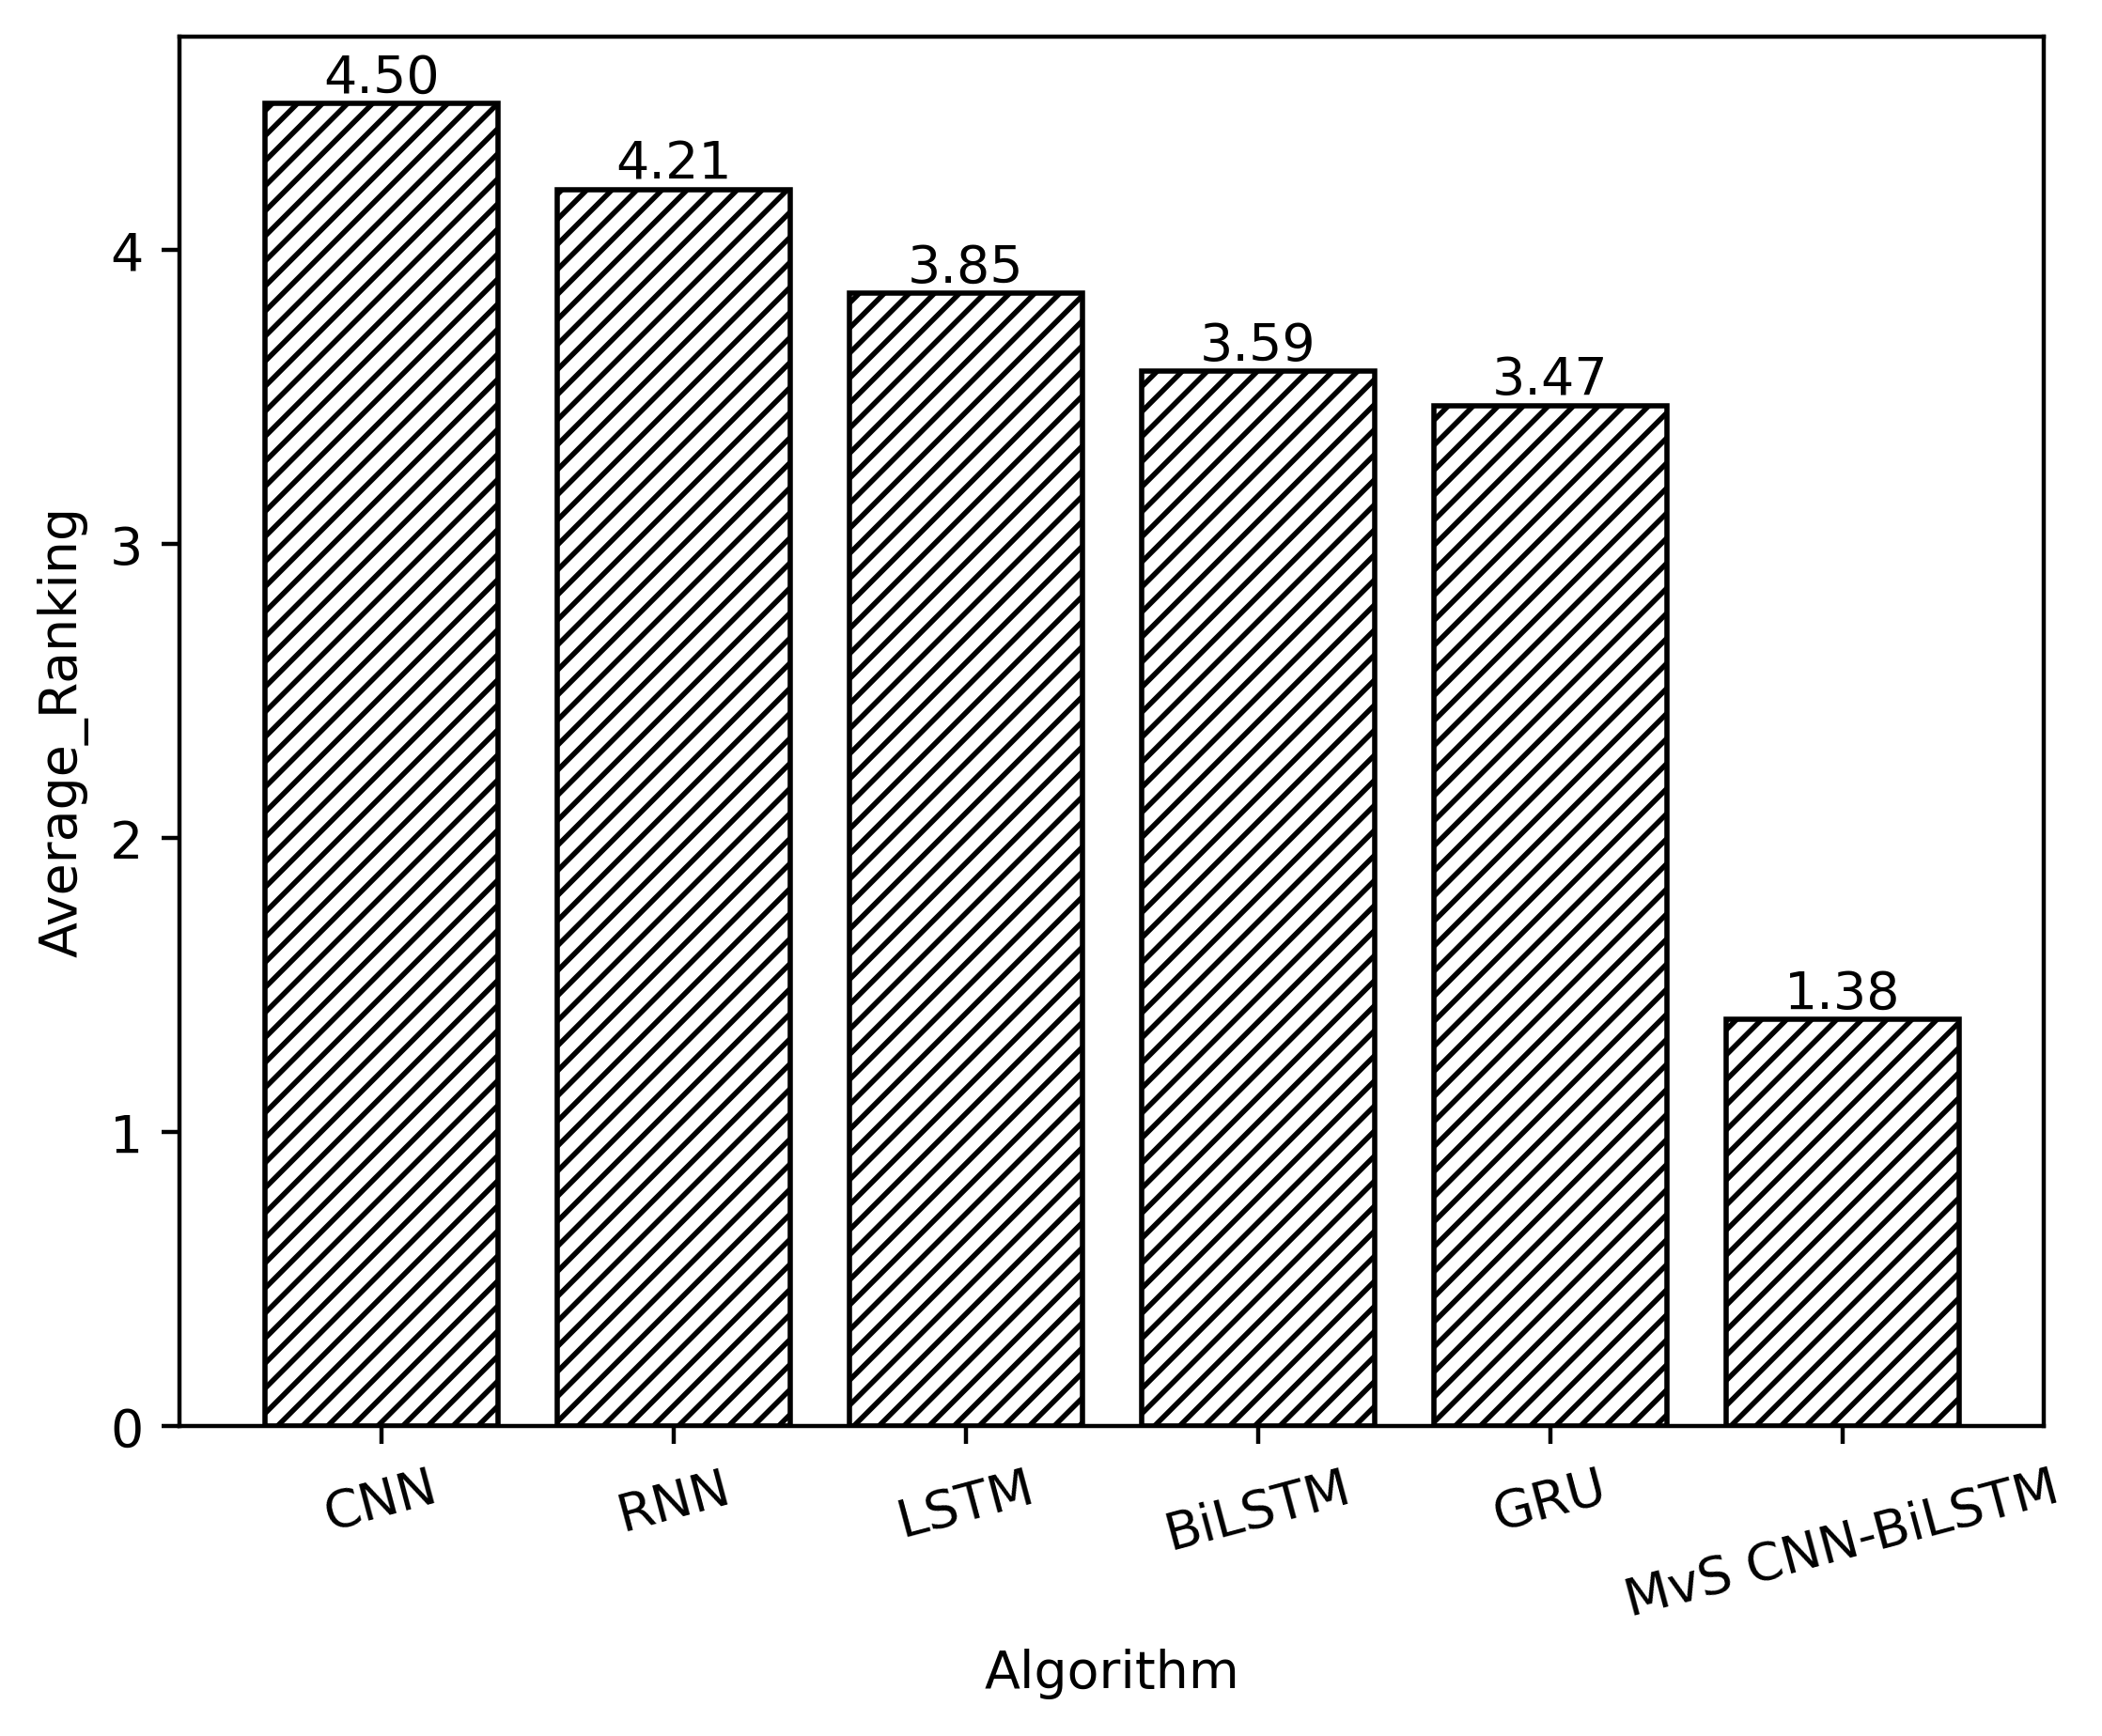
\includegraphics[scale=0.8]{avg_Rank_plot}
    \caption{Overall average Friedman ranking of traditional models and proposed MvS CNN-BiLSTM model.}
    \label{avg_Rank_plot}
  \end{figure*}
  In \Cref{AVG RANK},  the mean rankings of various algorithms are presented according to their performance on two performance metrics,  namely RMSE and MAPE. The table also includes an additional column for the average ranking across both metrics. The initial column suggests the average positions of each formula based on their RMSE performance. In contrast, the second column displays the average positions of each formula based on their MAPE performance. The third column signifies the mean rank of each algorithm,  factoring in performance on both metrics and providing a comprehensive measure of performance. In \Cref{AVG RANK} show average ranking on both performance measures and concluded the best algorithm. The underperformance of conventional deep learning structures such as BiLSTM,  CNN,  GRU,  LSTM,  and RNN,  despite their higher ranking on average,  is a surprising observation compared to the MvS CNN-BiLSTM method. Thus,  according to \Cref{avg_Rank_plot}, the mean ranking over the two performance metrics,  the MvS CNN-BiLSTM algorithm is regarded as the optimal algorithm out of all the models. The bar graph provided is illegible and cannot be used to support the previous analysis,  showing that the MvS CNN-BiLSTM algorithm has no ranking or comparison to the traditional deep learning models (BiLSTM,  CNN,  GRU,  LSTM,  and RNN) on average for the given task. The CNN and RNN algorithms were rated the worst on average,  suggesting their performance was not as great as other models.



